\documentclass[11pt,a4paper]{article}

\usepackage{amsfonts,amsmath,amssymb,amsthm}
\usepackage[utf8]{inputenc}
\usepackage[T1]{fontenc}
\usepackage[francais]{babel}
\usepackage{mathptmx}
\usepackage{fancybox}
\usepackage{graphicx}
\usepackage{ifthen}

\usepackage{tikz}   

\usepackage{hyperref}
\hypersetup{colorlinks=true, linkcolor=blue, urlcolor=blue,
	pdftitle={Exo7 - Exercices de mathématiques}, pdfauthor={Exo7}}

\usepackage{geometry}
\geometry{top=2cm, bottom=2cm, left=1cm, right=1cm}



\begin{document}


\section{Dupuy}

\begin{figure*}[!h]
	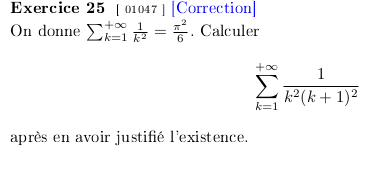
\includegraphics[scale=0.8]{1.png}
\end{figure*}

\begin{figure*}[!h]
	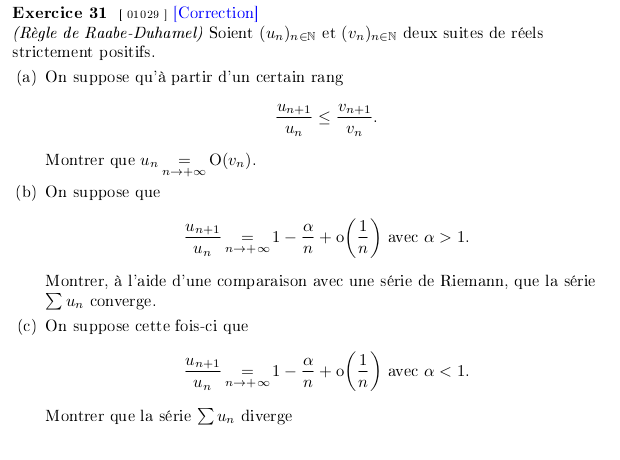
\includegraphics[scale=0.8]{2.png}
\end{figure*}

\begin{figure*}[!h]
	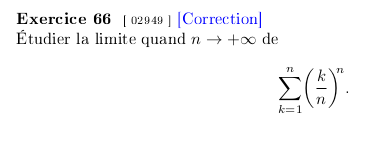
\includegraphics[scale=0.8]{3.png}
\end{figure*}


\newpage
\section{Mansuy}

\begin{figure*}[!h]
	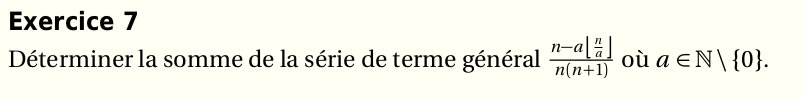
\includegraphics[scale=0.6]{4.png}
\end{figure*}

\begin{figure*}[!h]
	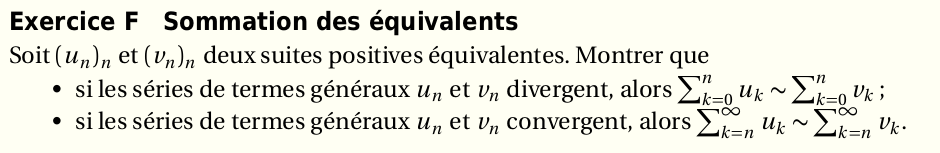
\includegraphics[scale=0.6]{5.png}
\end{figure*}
\newpage



\title{
	1 Dupuy
}

Exercice 25 [ 01047] [Correction] On donne $\sum_{k=1}^{+\infty} \frac{1}{k^{2}}=\frac{\pi^{2}}{6}$. Calculer

$$
\sum_{k=1}^{+\infty} \frac{1}{k^{2}(k+1)^{2}}
$$

après en avoir justifié l'existence.\\

Exercice 31 [ 01029 ] [Correction]

(Règle de Raabe-Duhamel) Soient $\left(u_{n}\right)_{n \in \mathbb{N}}$ et $\left(v_{n}\right)_{n \in \mathbb{N}}$ deux suites de réels strictement positifs.

(a) On suppose qu'à partir d'un certain rang

$$
\frac{u_{n+1}}{u_{n}} \leq \frac{v_{n+1}}{v_{n}} .
$$

Montrer que $u_{n} \underset{n \rightarrow+\infty}{=} \mathrm{O}\left(v_{n}\right)$.

(b) On suppose que

$$
\dfrac{u_{n+1}}{u_{n}} \underset{n \rightarrow+\infty}{=} 1-\dfrac{\alpha}{n}+o\left(\frac{1}{n}\right) \text { avec } \alpha>1 .
$$

Montrer, à l'aide d'une comparaison avec une série de Riemann, que la série $\sum u_{n}$ converge.

(c) On suppose cette fois-ci que

$$
\frac{u_{n+1}}{u_{n}} \underset{n \rightarrow+\infty}{=} 1-\frac{\alpha}{n}+o\left(\frac{1}{n}\right) \text { avec } \alpha<1 .
$$

Montrer que la série $\sum u_{n}$ diverge

Exercice 66 [ 02949 ] [Correction]

Étudier la limite quand $n \rightarrow+\infty$ de

$$
\sum_{k=1}^{n}\left(\frac{k}{n}\right)^{n} .
$$



\section{Mansuy}

\section{Exercice 7}

Déterminer la somme de la série de terme général $\frac{n-a\left\lfloor\frac{n}{a}\right\rfloor}{n(n+1)}$ où $a \in \mathbb{N} \backslash\{0\}$.

\section{Exercice $\mathbf{F}$ Sommation des équivalents}

Soit $\left(u_{n}\right)_{n}$ et $\left(v_{n}\right)_{n}$ deux suites positives équivalentes. Montrer que

- si les séries de termes généraux $u_{n}$ et $v_{n}$ divergent, alors $\sum_{k=0}^{n} u_{k} \sim \sum_{k=0}^{n} v_{k}$;

- si les séries de termes généraux $u_{n}$ et $v_{n}$ convergent, alors $\sum_{k=n}^{\infty} u_{k} \sim \sum_{k=n}^{\infty} v_{k}$.
\end{document}
